\documentclass[border=3mm]{standalone}

\usepackage{tikz}
\usetikzlibrary{arrows.meta}

\begin{document}
	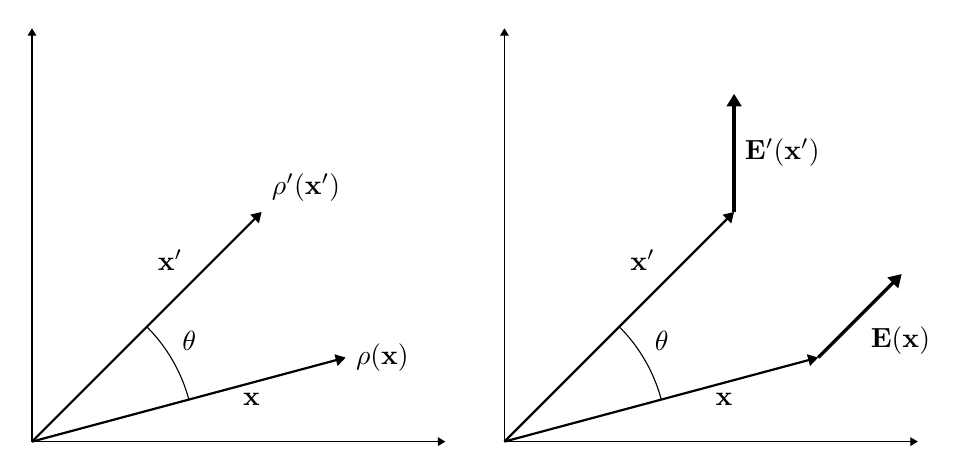
\begin{tikzpicture}[scale=1.5]
		%% Left figure
		\draw[-{Triangle[scale=0.75]}] (0,0) coordinate (o) -- (3.5,0);
		\draw[-{Triangle[scale=0.75]}] (o) -- (0,3.5);
		\draw[thick,-{Triangle[scale=0.75]}] (o) --++ (15:2.75cm) coordinate[pos=.5] (a) node[pos=0.7,below]{$\mathbf{x}$} node[right]{$\rho(\mathbf{x})$};
		\draw[thick,-{Triangle[scale=0.75]}] (o) --++ (45:2.75cm)node[pos=0.7,above left]{$\mathbf{x'}$} node[above right]{$\rho'(\mathbf{x'})$};
		\draw (a) arc (15:45:1.375cm) node[midway,above right]{$\theta$};
		
		% Right figure
		\begin{scope}[xshift=4cm]
			\draw[-{Triangle[scale=0.75]}] (0,0) coordinate (o) -- (3.5,0);
			\draw[-{Triangle[scale=0.75]}] (o) -- (0,3.5);
			\draw[thick,-{Triangle[scale=0.75]}] (o) --++ (15:2.75cm) coordinate[pos=.5] (a) node[pos=0.7,below]{$\mathbf{x}$} coordinate (1);
			\draw[thick,-{Triangle[scale=0.75]}] (o) --++ (45:2.75cm)node[pos=0.7,above left]{$\mathbf{x'}$} coordinate (2);
			\draw (a) arc (15:45:1.375cm) node[midway,above right]{$\theta$};
			\draw[very thick,-{Triangle[scale=0.75]}] (1) --++ (45:1cm) node[midway,below right] {$\mathbf{E(x)}$};
			\draw[very thick,-{Triangle[scale=0.75]}] (2) --++ (90:1cm) node[midway,right] {$\mathbf{E'(x')}$};
		\end{scope}
	\end{tikzpicture}
\end{document}